% ENCODER --------------------------------
\section{Architecture for DUMs}
\label{sec:architecture}

In this section, we study the impact of the architecture component in DUMs. To this end, we look at different \emph{latent dimensions}, different \emph{architectural types and size}, and applying different \emph{regularization constraints} to avoid \textit{feature collapse} \citep{van2021due}. 

\textbf{Latent dimension.} We vary the dimension of the output space of the core architecture. We show the results for each pair of ID dataset and its distribution shifted OOD dataset (MNIST/CMNIST, CIFAR/CIFAR-C, CamelyonID/CamelyonOOD) with the core architecture ResNet18 for MNIST/CIFAR, and WideResNet-28-10 for Camelyon in \cref{fig:latent} and additional uncertainty estimation results in the appendix \cref{fig:latent_ood}. \underline{\textit{Observation:}} We observe that increasing the latent dimensions leads to improvement for DUMs on ID and OOD datasets with particularly significant improvement for NatPN (see \cref{fig:latent}). This suggests that higher latent dimensions are more expressive by encoding more information. However, we observe that  a too high latent dimension can degrade OOD detection performance by causing numerical instabilities in the training (see \cref{fig:latent_ood}), suggesting a trade-off between OOD generalization and OOD detection.

\begin{figure}[!htb]
    \centering
    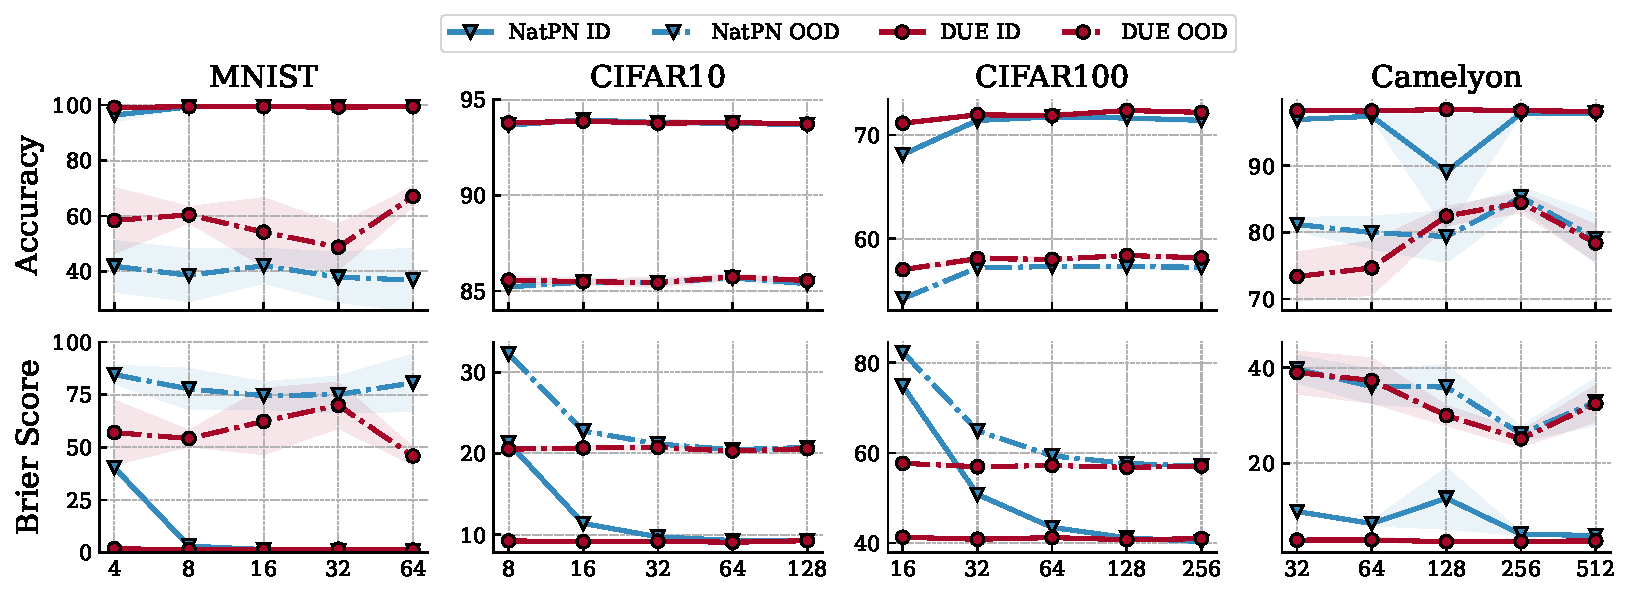
\includegraphics[width=0.9\textwidth]{sections/008_iclr2023/figures/latent.pdf}
    \caption{Results of DUMs when varying the \textbf{latent dimension size}. We observe that increasing the latent dimension consistently leads to similar or better predictive performance.}
    \label{fig:latent}
\end{figure}
    % We observe that increasing the latent dimension can increase the predictive performance.}

\textbf{Architecture type and size.} We compare the influence of the type and size of the core architecture on the performance of DUMs. We consider residual, convolutional, and transformer architectures like ResNet18, ResNet50, EfficientNetV2, and Swin \citep{he2016resnet, tan2021effcientnet, liu2021swin}. We show the results for DUMs trained on CIFAR100 as ID with the different core architectures in \cref{tab:encoder_architecture} and additional results at appendix \cref{tab:encoder_architecture_ood}. \underline{\textit{Observation:}} We observe that models with more parameters achieve better results. In particular, ResNet50 achieves significantly better results than ResNet18. Further, more recent core architectures like EfficientNetV2 and Swin are better calibrated and more expressive leading to a better overall performance. This can be explained by the fact that they are more expressive and provide more informative embeddings for the uncertainty head to operate on. This aligns with \citet{minderer2021calibration} which states that the architecture type is important for the calibration properties. 

% \begin{wraptable}{r}{0.5\textwidth}
% \centering
% \caption{\textbf{Encoder Architecture Comparison.} Recent architectures are better calibrated with similar or better uncertainty estimation. The reported OOD results are an average over all the independent OOD dataset result.}
% \label{tab:encoder_architecture}
% \tiny
% \begin{tabular}{lcccccc}\toprule
% \textbf{Encoder} &\textbf{Param.} &\textbf{Brier Score} &\textbf{OOD Pred.} &\textbf{OOD Epis.} \\
% \midrule
% ResNet18 &11.6M &33.69 $\pm$ 0.15 &87.49 $\pm$ 1.90 &81.79 $\pm$ 1.38 \\
% ResNet50 &25.5M &23.67 $\pm$ 0.27 &84.95 $\pm$ 1.48 &89.08 $\pm$ 0.70 \\
% \textbf{EffNet\_V2\_S} &\textbf{21.4M} &\textbf{17.08 $\pm$ 0.10} &\textbf{87.79 $\pm$ 0.77} &89.47 $\pm$ 0.59 \\
% Swin\_T &28.2M &18.48 $\pm$ 0.06 &85.91 $\pm$ 1.17 &\textbf{90.23 $\pm$ 0.81} \\
% \midrule
% ResNet18 &11.6M &36.57 $\pm$ 0.15 &88.04 $\pm$ 0.67 &- \\
% ResNet50 &25.5M &28.09 $\pm$ 0.19 &\textbf{90.24 $\pm$ 0.51} &- \\
% \textbf{EffNet\_V2\_S} &21.4M &\textbf{21.07 $\pm$ 0.06} &89.43 $\pm$ 0.67 &- \\
% Swin\_T &28.2M &23.23 $\pm$ 0.05 &89.90 $\pm$ 0.36 &- \\
% \bottomrule
% \end{tabular}
% \end{wraptable}

\begin{table}[!htp]\centering
\caption{Results of DUMs for different \textbf{architecture types.} including residual, convolutional, and transformer architectures on CIFAR100.  OOD results are averaged over OOD datasets. Bold numbers indicate best results among all settings. Larger and more recent architectures are better calibrated with similar or better uncertainty estimation.}
\label{tab:encoder_architecture}
\tiny

\resizebox{0.9\textwidth}{!}{%
\begin{tabular}{llcccccc}\toprule
\textbf{Method} &\textbf{Architecture} &\textbf{\#Parameters} &\textbf{Accuracy ($\uparrow$)} &\textbf{Brier Score ($\downarrow$)} &\textbf{OOD Pred. ($\uparrow$)} &\textbf{OOD Epis. ($\uparrow$)} \\
\midrule
\multirow{4}{*}{NatPN} &ResNet18 &11.6M &80.31 $\pm$ 0.09 &33.69 $\pm$ 0.15 &87.49 $\pm$ 1.90 &81.79 $\pm$ 1.38 \\
&ResNet50 &25.5M &84.22 $\pm$ 0.12 &23.67 $\pm$ 0.27 &84.95 $\pm$ 1.48 &89.08 $\pm$ 0.70 \\
&EffNet\_V2\_S &21.4M &\textbf{88.43 $\pm$ 0.10} &\textbf{17.08 $\pm$ 0.10} &\textbf{87.79 $\pm$ 0.77} &89.47 $\pm$ 0.59 \\
&Swin\_T &28.2M &87.99 $\pm$ 0.09 &18.48 $\pm$ 0.06 &85.91 $\pm$ 1.17 &\textbf{90.23 $\pm$ 0.81} \\
\midrule
\multirow{4}{*}{DUE} &ResNet18 &11.6M &78.85 $\pm$ 0.19 &36.57 $\pm$ 0.15 &88.04 $\pm$ 0.67 &- \\
&ResNet50 &25.5M &82.42 $\pm$ 0.14 &28.09 $\pm$ 0.19 &\textbf{90.24 $\pm$ 0.51} &- \\
&EffNet\_V2\_S &21.4M &86.92 $\pm$ 0.08 &\textbf{21.07 $\pm$ 0.06} &89.43 $\pm$ 0.67 &- \\
&Swin\_T &28.2M &\textbf{86.93 $\pm$ 0.05} &23.23 $\pm$ 0.05 &89.90 $\pm$ 0.36 &- \\
\bottomrule
\end{tabular}
}
\end{table}

\textbf{Regularization constraints.} \emph{Feature collapse} is a phenomenon where a model may discard important parts of the input information during its training phase, which may degrade OOD detection performance \citep{van2021due}. Two techniques to avoid feature collapses are \textit{bi-Lipschitz} constraints via combining residual connections and lipschitz constraints \citep{liu2020sngp}, and \textit{reconstruction} constraints via adding an additional reconstruction term in the loss \citep{postels2020reconstruction}. We show the results for DUMs trained on the datasets MNIST and CIFAR100 with ResNet18 in \cref{fig:bi,fig:rec} and additional results for other datasets (Toy dataset, CIFAR10, Camelyon) at \cref{subsec:appendix_encoder}. \underline{\textit{Observation:}} We observe that the reconstruction technique is not capable to avoid feature collapse. Indeed, we show  that, even with reconstruction constraints, some (non-discriminative) features can completely collapse (see \cref{fig:rec_toy_collapse,fig:rec_toy} for toy examples). Hence, while this method can lead to small OOD improvements on simple tasks (see e.g. MNIST in \cref{fig:rec}), this benefit does not generalize to more complex tasks (see e.g. CIFAR100 in \cref{fig:rec}). In contrast, we observe that bilipschitz constraints indeed mitigate the collapse of features (see \cref{fig:bi_toy_collapse,fig:bi_toy} for toy examples), leading to similar or higher OOD detection performance (see \cref{fig:bi}). The mitigation of feature collapse can be mostly assigned to the residual connection constraints. However, bilipschitz constraints can improve OOD detection results on simple tasks (e.g. MNIST, CIFAR10), it degrades OOD generalization performance (see \cref{fig:bi}) and does not significantly improve OOD detection on more complex tasks (see e.g. Camelyon, CIFAR100 in \cref{fig:bi_bar_full}). Intuitively, maintaining features which are not discriminative to the task might introduce spurious correlations, thus degrading performances. E.g. enforces the architecture to encode the color feature in the latent space decreases the performance of the OOD CMNIST datasets after training on the ID MNIST dataset. 

\begin{figure}
\begin{minipage}[t]{0.48\textwidth}
    \centering
    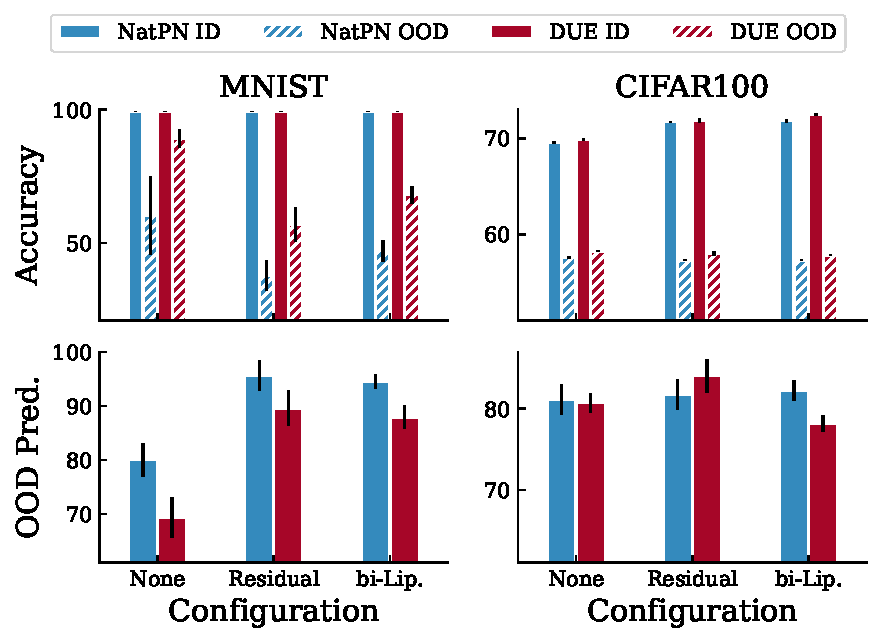
\includegraphics[width=0.9\textwidth]{sections/008_iclr2023/figures/bi_bar_short.pdf}
    \caption{Results OOD generalization and detection of DUMs with none, residual and bi-lipschitz \textbf{architecture constraints} on MNIST/CMNIST and CIFAR/CIFAR-C. Bi-lipschitz can improve OOD detection by mitigating feature collapse (see \cref{fig:bi_toy}) at the expense of degrading OOD generalization.}
    \label{fig:bi}
\end{minipage}\quad%
%
\begin{minipage}[t]{0.48\textwidth}
    \centering
    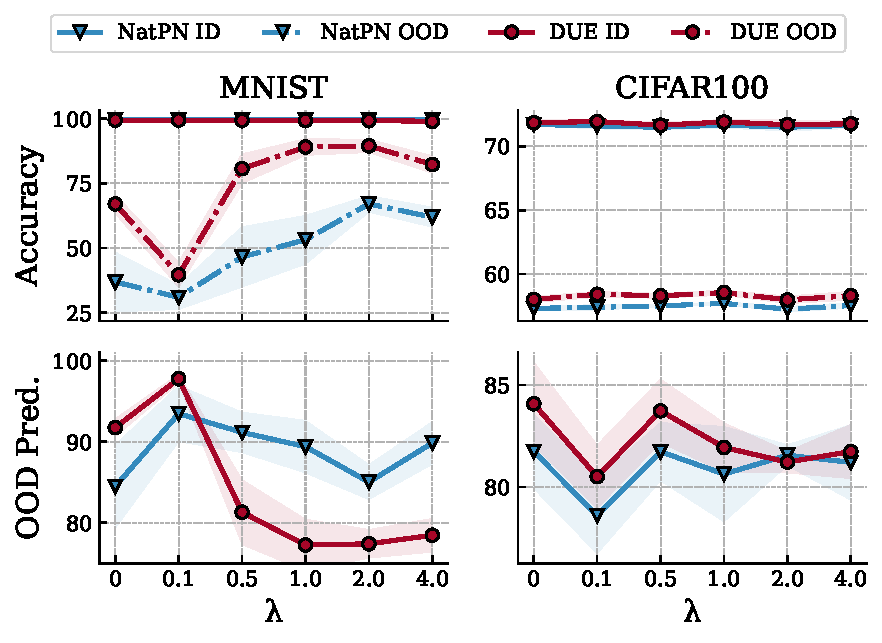
\includegraphics[width=0.9\textwidth]{sections/008_iclr2023/figures/reconst_short.pdf}
    \caption{Results OOD generalization and detection of DUMs with reconstruction \textbf{architecture constraints} on MNIST/CMNIST and CIFAR/CIFAR-C. Increasing the reconstruction strength $\lambda$ improves the OOD generalization on simple MNIST/CMNIST dataset but fails for complex datasets. Reconstruction fails to improve OOD detection since it does not avoid feature collapse (see \cref{fig:rec_toy}). }
    \label{fig:rec}
\end{minipage}
\end{figure}
